\documentclass[]{article}
\usepackage[latin1]{inputenc}
\usepackage{tikz}
\usetikzlibrary{shapes,arrows}

	\pagestyle{empty}
	
	
	% Define block styles
	\tikzstyle{decision} = [diamond, draw, fill=blue!20, 
	text width=20em, text badly centered, node distance=3cm, inner sep=0pt]
	\tikzstyle{block} = [rectangle, draw, fill=red!20, 
	text width=20em, text centered, rounded corners, minimum height=4em]
	\tikzstyle{line} = [draw, -latex']
	\tikzstyle{cloud} = [draw, ellipse,fill=red!20, node distance=3cm, minimum height=2cm]

%opening
\title{A SEMI-AUTOMATIC MACHINE TO CLEAN SEWER WASTE AND BY PRODUCTS FROM THE WASTE}
\author{}

\begin{document}

\maketitle



\section{Introduction/ Motivation:}
\subparagraph{We know that manual scavenging is not a good practice to clean drains. But it is very common to see a person, who dip in the drain to clean it. Due to that many sewer cleaners face different types of diseases. Many of them died due to exposure of harmful gases. Other than that, the waste produced are collected and hip of waste are dumped in the outskirts of the city. Which produce a large amount of methane gas. }
\paragraph{}
To avoid cleaning drains manually a semi-automatic machine is used by the sewer cleaners which help them to clean the drains. Due to this the cleaner would not have to dip in the drain. Also, they dont have to face any diseases. On the other hand, rather staging the huge hip of wastes we can able to produce methane gas from that and using it as a flammable fuel. And the plastics obtained from the wastes, are used to make roads.

\begin{center}
	\includegraphics[scale=0.7]{C:/Users/DELL/Downloads/drain}
\end{center}
	
\section{Market Research/Literature Survey:}
\subparagraph{}
To avoid manual scavenging an automatic robot is introduced earlier. It is done in Greater Hyderabad Municipal Corporation (GHMC) to clean manholes. The robot is consisting of hands, legs and a bucket of 18 litre. The hand goes inside the manhole. The legs help the robot to reach the waste. And the bucket is used to carry out the waste which is collected
\paragraph{}
The robot is also consisting of many other parts such as various sensors to measure environmental parameters, temperature of the manhole, size of the manhole, etc. A camera is also installed in the robot to observe during night. 


\section{Hardware requirements:}
\subparagraph{(a)motors}
\subparagraph{(b)jumper wires}
\subparagraph{(c)motor driver}
\subparagraph{(d)arduino uno}
\subparagraph{(e)transmitter/receiver}
\subparagraph{(f)aluminium sheet}
\subparagraph{(g)netplate}

\section{Software requirements:}
\subparagraph{(a)arduino droid}
\subparagraph{}
\paragraph{}

\section{Secification}
\paragraph{}
The machine is a semi-automatic machine. which is controlled by the cleaner. It consist of motors, arduino uno, bucket, jumper wires to connect the components and motor driver to controll motors. The software requirements is arduino droid.

\section{Project cost}
\paragraph{}
the projects cost may be near about 15000 rupess 
 
\section{Work distribution}
\paragraph{}
mechanical works in the projects is done by Suraj parasad
\paragraph{}
programs in the project is done by Avishek bhadra
\paragraph{}
production of by products from waste is done by Souvik chakraborty
\paragraph{}
the machine is controlled by Amrita sain
 
\section{Implementation:}
\paragraph{}
A machine which is operated by the sewer cleaners, is taken and installed in the track which is developed in the drain. After fixing the machine in the track, an aluminium bucket is ready to dip in the drain to take all the waste out. After doing this the machine is ready to clean the drain. When the bucket is filled the bucket moves 90degree and it came out from the drain. After coming out the sewer cleaner make the bucket an air tight container. And the container is taken up, to produce methane gas from the waste as by product. After producing methane gas, the residue is used as manure. And the plastic materials obtained from the waste is used to build roads.

\paragraph{}
Motor driver:	Some motors are required to make the machine movable. In some parts stepper motors are used. To operate stepper motor, a motor driver is needed. It is used to control the torque of motor. Specially used for stepper motor. It is connected with the stepper motor and the Arduino. It gets instruction from the Arduino and drives the motor as per requirements. 

\paragraph{}
Arduino UNO: It is installed between the receiver and the motor driver. The Arduino takes the input signal from the receiver and processed himself according to input signal. It controls the motor driver according to the signal. 	Other than that, the Arduino can also be used to make the machine automatic in future if needed. The only thing is to program the UNO perfectly.

\section{User interface:}
\paragraph{}
The machine set is consisting of the machine part and a transmitter. The user (sewer cleaner) will first have to charge the machine part and the transmitter part properly. After charging it for about 4hrs, the user can able to use it. Now the user has to switch on the machine and the transmitter. After that controls the machine with the help of transmitter. The user will drive the machine by the transmitter in his hand. When the machine is installed in the drain and the bucket is ready to dip in the drain, the user with help of transmitter will control the machine as well as the bucket. When the bucket is filled up with waste it is taken out and transformed into an air tight container for further process.
\section{Flow chart:}
\paragraph{}
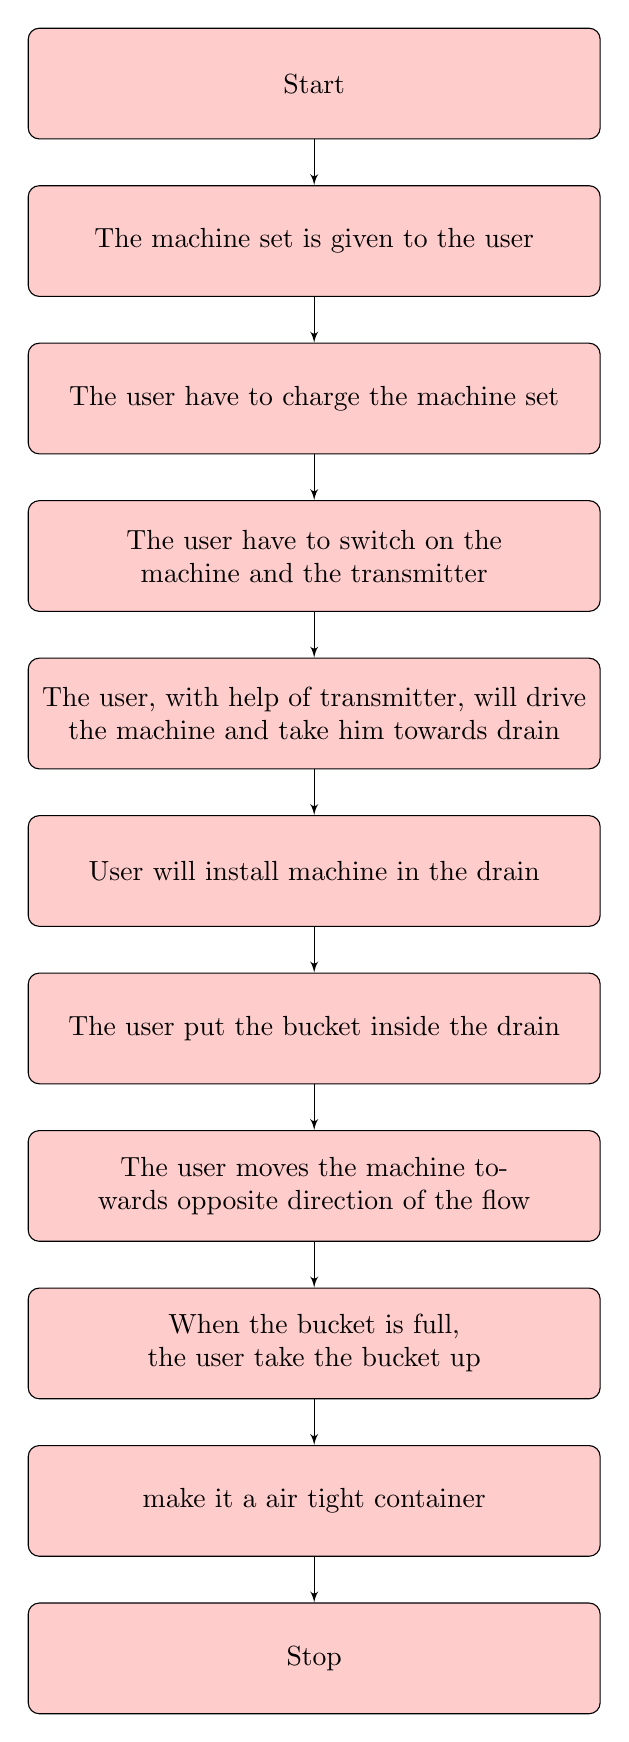
\begin{tikzpicture}[node distance = 2cm, auto]
	% Place nodes
	\node [block] (init) {Start};
	\node [block, below of=init] (identify) {The machine set is given to the user };
	\node [block, below of=identify] (evaluate) {The user have to charge the machine set};
	\node [block, below of=evaluate] (decide) {The user have to switch on the machine and the transmitter};
	\node [block, below of=decide] (user) {The user, with help of transmitter, will drive the machine and take him towards drain };
	\node [block, below of=user] (install) {User will install machine in the drain };
	\node [block, below of=install] (put) {The user put the bucket inside the drain };
	\node [block, below of=put] (moves) {The user moves the machine towards opposite direction of the  flow };
	\node [block, below of=moves] (bucket) {When the bucket is full, the user take the bucket up };
	\node [block, below of=bucket] (container) {make it a air tight container};
	\node [block, below of=container] (stop) {Stop};
	% Draw edges
	\path [line] (init) -- (identify);
	\path [line] (identify) -- (evaluate);
	\path [line] (evaluate) -- (decide);
	\path [line] (decide) -- (user);
	\path [line] (user) -- (install);
	\path [line] (install) -- (put);
	\path [line] (put) -- (moves);
	\path [line] (moves) -- (bucket);
	\path [line] (bucket) -- (container);
	\path [line] (container) -- (stop);
	\end{tikzpicture}

\section{Feasibility:}
\paragraph{}
Now a day in many areas the sewer cleaner would not able to reach the waste in the drain. And because of that they have to dip in the drain. To avoid this a robot is made which helps the worker to clean manholes. But there are many places where there are still open drains. Other than that, the cost of that robot is too much. So, to reduce all the limitations we are trying to make a semi-automatic machine which will help the sewer cleaners.

\end{document}
